% IEEE conference paper for Land Registry Management System (LRMS)
% Compile with: pdflatex lrms_ieee.tex; bibtex lrms_ieee; pdflatex; pdflatex
\documentclass[conference]{IEEEtran}

% Packages
\usepackage{cite}
\usepackage{graphicx}
\usepackage{booktabs}
\usepackage{amsmath}
\usepackage{hyperref}
\usepackage{xcolor}
\usepackage{listings}
\usepackage{tikz}
\usetikzlibrary{arrows.meta, positioning}

% Listings setup (for SQL and code)
\lstdefinestyle{lrms}{
  basicstyle=\ttfamily\footnotesize,
  numbers=left,
  numberstyle=\tiny, numbersep=6pt,
  frame=single,
  breaklines=true,
  keywordstyle=\color{blue!70!black},
  commentstyle=\color{green!50!black},
  stringstyle=\color{red!60!black},
}
\lstset{style=lrms}

% Hyperref setup
\hypersetup{
  colorlinks=true,
  linkcolor=blue,
  citecolor=blue,
  urlcolor=blue
}

\begin{document}

\title{An Enterprise-Grade Land Registry Management System Using Flask and MySQL with Advanced Database Features}

\author{\IEEEauthorblockN{Abhijeet Nardele}
\IEEEauthorblockA{Department of Computer Engineering\\
[Your Institution Name]\\
Email: abhijeet.nardele@example.com}}

\maketitle

\begin{abstract}
Digitizing land records is critical for governance, transparency, and citizen services. This paper presents the design and implementation of a Land Registry Management System (LRMS) built with Flask (Python) and MySQL. The system supports role-based workflows for administrators, registrars, officers, and citizens, covering property registration, ownership management, mutations, tax assessment and payments, document handling, notifications, and audit logging. A key contribution is the use of advanced MySQL features—stored procedures, triggers, views, and strategic indexing—to enforce business rules at the database layer and improve performance. We integrate interactive mapping with Leaflet and analytics with Chart.js. We describe the architecture, schema, security controls, implementation details, and validation on a realistic dataset. The solution demonstrates a production-ready blueprint for e-governance land registry systems.
\end{abstract}

\begin{IEEEkeywords}
Land registry, DBMS, Flask, MySQL 8.0, Stored procedures, Triggers, Views, GIS, Leaflet, RBAC, E-governance
\end{IEEEkeywords}

\section{Introduction}
Land records underpin taxation, ownership security, and public services. Legacy manual processes are error-prone and slow, while modern e-governance requires robust, auditable, and secure systems. We present LRMS, a web-based system implementing end-to-end workflows: property registration with ULPIN generation, ownership and joint-ownership, mutation processing, tax assessment and payments, document management, notifications, and comprehensive audit trails.

\textbf{Contributions:}
\begin{itemize}
  \item An end-to-end LRMS with role-based access control (Admin, Registrar, Officer, Citizen) implemented in Flask and SQLAlchemy.
  \item Advanced MySQL layer: four production-ready stored procedures, four triggers, seven views, and indexing strategy for performance.
  \item GIS-enabled features using Leaflet for property geolocation and visualization.
  \item Security hardening: password hashing, CSRF protection, RBAC, validated uploads, and audit logging.
  \item Validation on a realistic dataset with automated tests and sample workflows.
\end{itemize}

\section{Background and Related Work}
Government initiatives are adopting unique land parcel identifiers (e.g., ULPIN) and digitized registries to improve transparency. Commercial platforms and academic prototypes often emphasize either frontend usability or backend data quality. Our approach emphasizes moving business logic into the database via stored programs and triggers for consistency and auditability, while keeping the application service layer clean and maintainable.

\section{System Overview and Architecture}
Fig.~\ref{fig:arch} shows a classic three-tier architecture: a Flask web application (Blueprints for roles and APIs), a MySQL 8.0 database with advanced features, and a browser client with Bootstrap, Chart.js, and Leaflet.

\begin{figure}[t]
  \centering
  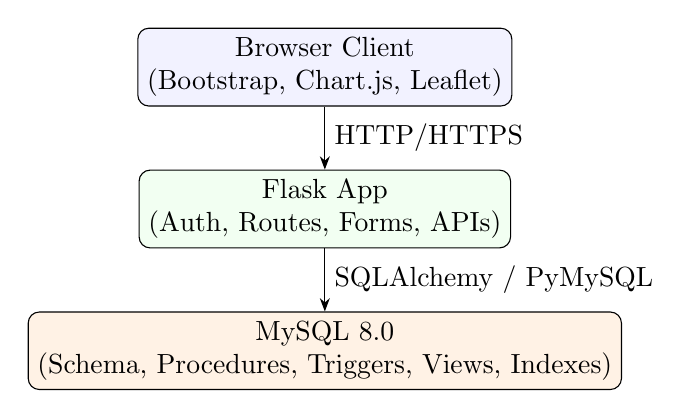
\begin{tikzpicture}[node distance=8mm and 10mm, >=Stealth]
    % Nodes
    \node[draw, rounded corners, fill=blue!5, align=center] (client) {Browser Client\\(Bootstrap, Chart.js, Leaflet)};
    \node[draw, rounded corners, fill=green!5, align=center, below=of client] (flask) {Flask App\\(Auth, Routes, Forms, APIs)};
    \node[draw, rounded corners, fill=orange!10, align=center, below=of flask] (db) {MySQL 8.0\\(Schema, Procedures, Triggers, Views, Indexes)};

    % Arrows
    \draw[->] (client) -- node[right]{HTTP/HTTPS} (flask);
    \draw[->] (flask) -- node[right]{SQLAlchemy / PyMySQL} (db);
  \end{tikzpicture}
  \caption{LRMS architecture.}
  \label{fig:arch}
\end{figure}

\noindent\textbf{Roles and capabilities} are summarized in Table~\ref{tab:roles}.

\begin{table}[t]
  \centering
  \caption{Roles and key capabilities}
  \label{tab:roles}
  \begin{tabular}{@{}ll@{}}
    \toprule
    Role & Selected capabilities \\
    \midrule
    Administrator & User mgmt, reports, settings \\
    Registrar & Approve registrations, certificates \\
    Officer & Review/approve mutations \\
    Citizen & Register properties, mutations, payments \\
    \bottomrule
  \end{tabular}
\end{table}

\section{Database Design}
The schema centers on \texttt{users}, \texttt{properties}, \texttt{owners}, \texttt{ownerships} (many-to-many), \texttt{mutations}, \texttt{payments}, \texttt{documents}, \texttt{notifications}, \texttt{audit\_logs}, and \texttt{tax\_assessments}. Keys, constraints, and indexes are defined for integrity and performance (e.g., unique \texttt{email}, \texttt{ulpin}; FKs between ownerships, properties, owners). ULPIN supports unique parcel identification.

We employ strategic indexes (e.g., on \texttt{status}, \texttt{ulpin}, location columns) to accelerate dashboards, search, and approval queues. Views provide denormalized, read-optimized projections for reporting.

\textbf{Sample dataset:} 70+ users across roles, 10+ properties and mutations, payments, and audit trails to validate end-to-end workflows.

\begin{figure}[t]
  \centering
  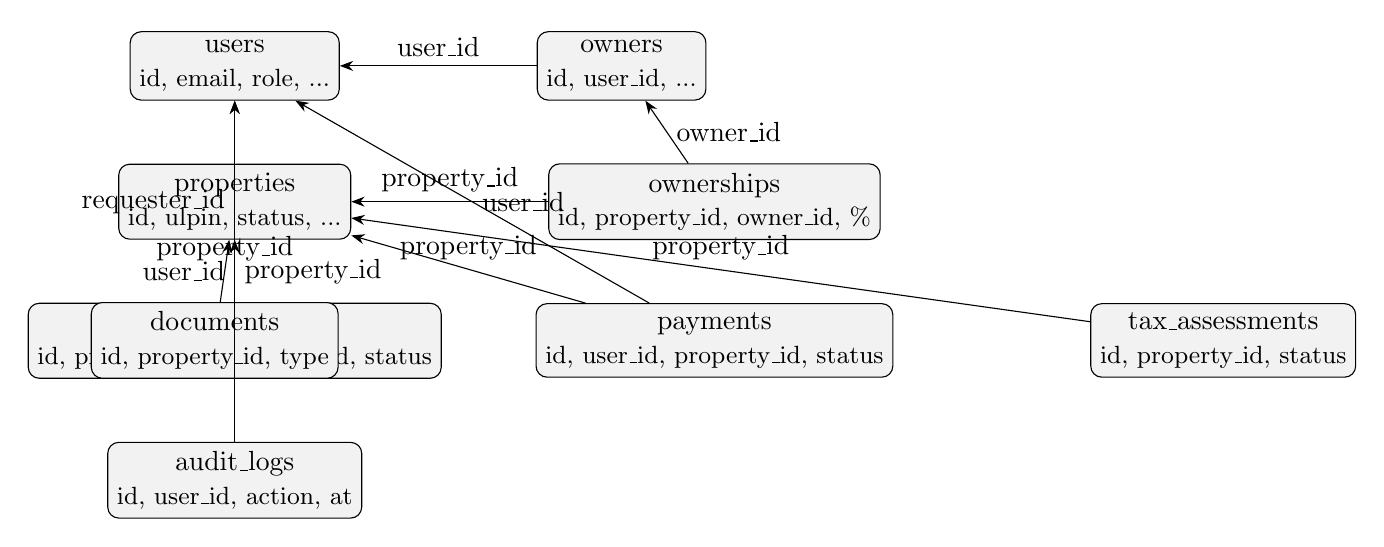
\begin{tikzpicture}[node distance=8mm and 10mm, >=Stealth]
    % Tables
    \node[draw, rounded corners, fill=gray!10, align=center] (users) {users\\\small id, email, role, ...};
    \node[draw, rounded corners, fill=gray!10, align=center, right=25mm of users] (owners) {owners\\\small id, user\_id, ...};
    \node[draw, rounded corners, fill=gray!10, align=center, below=of users] (properties) {properties\\\small id, ulpin, status, ...};
    \node[draw, rounded corners, fill=gray!10, align=center, right=25mm of properties] (ownerships) {ownerships\\\small id, property\_id, owner\_id, \%};
    \node[draw, rounded corners, fill=gray!10, align=center, below=of properties] (mutations) {mutations\\\small id, property\_id, requester\_id, status};
    \node[draw, rounded corners, fill=gray!10, align=center, below=of ownerships] (payments) {payments\\\small id, user\_id, property\_id, status};
    \node[draw, rounded corners, fill=gray!10, align=center, below=of mutations] (audit) {audit\_logs\\\small id, user\_id, action, at};
    \node[draw, rounded corners, fill=gray!10, align=center, right=25mm of payments] (tax) {tax\_assessments\\\small id, property\_id, status};
    \node[draw, rounded corners, fill=gray!10, align=center, left=25mm of payments] (docs) {documents\\\small id, property\_id, type};

    % Relationships (FKs)
    \draw[-{Stealth}] (owners) -- node[above]{user\_id} (users);
    \draw[-{Stealth}] (ownerships) -- node[right]{owner\_id} (owners);
    \draw[-{Stealth}] (ownerships) -- node[above]{property\_id} (properties);
    \draw[-{Stealth}] (mutations) -- node[right]{property\_id} (properties);
    \draw[-{Stealth}] (mutations) -- node[left]{requester\_id} (users);
    \draw[-{Stealth}] (payments) -- node[right]{user\_id} (users);
    \draw[-{Stealth}] (payments) -- node[above]{property\_id} (properties);
    \draw[-{Stealth}] (docs) -- node[above]{property\_id} (properties);
    \draw[-{Stealth}] (audit) -- node[left]{user\_id} (users);
    \draw[-{Stealth}] (tax) -- node[above]{property\_id} (properties);
  \end{tikzpicture}
  \caption{Entity-Relationship overview of core LRMS tables.}
  \label{fig:erd}
\end{figure}

\section{Advanced MySQL Features}
We implement business logic in the database to improve correctness, observability, and performance.

\subsection{Stored Procedures}
\begin{itemize}
  \item \texttt{calculate\_property\_tax(property\_id, tax\_year)}: Computes tax by type and market value; inserts/updates tax assessment.
  \item \texttt{get\_property\_report(property\_id)}: Returns property, ownership, payment, and tax views.
  \item \texttt{get\_ownership\_chain(property\_id)}: Traverses ownership history.
  \item \texttt{get\_dashboard\_stats()}: Aggregates KPIs for dashboards.
\end{itemize}

\subsection{Triggers}
\begin{itemize}
  \item \texttt{after\_property\_insert}: Auto-generate ULPIN if absent.
  \item \texttt{before\_property\_update}: Log changes into \texttt{audit\_logs}.
  \item \texttt{after\_payment\_insert}: Update related tax assessment status.
  \item \texttt{after\_property\_status\_update}: Create notifications on approve/reject.
\end{itemize}

\subsection{Views and Indexing}
Seven views (e.g., \texttt{v\_property\_dashboard\_stats}, revenue and geographic summaries) support dashboards and analytics. Composite and full-text indexes accelerate common filters and searches.

\section{Methodology and Workflow}
The workflow comprises: (1) citizen registers property with geolocation; (2) registrar reviews and approves; (3) citizen submits mutation when ownership changes; (4) officer verifies and approves/rejects; (5) tax is assessed and payment recorded; (6) notifications and audit logs are generated automatically.

\section{Application Layer}
We adopt Flask Blueprints (\texttt{admin}, \texttt{registrar}, \texttt{officer}, \texttt{citizen}, \texttt{auth}, \texttt{api}) with SQLAlchemy ORM, Flask-Login, and WTForms. The UI uses Bootstrap 5, with charts via Chart.js and interactive property maps via Leaflet (including geolocation and draggable markers). Documents are securely uploaded with validation; reports can be exported to PDF (WeasyPrint/ReportLab) and Excel.

\section{Security}
Security controls include password hashing, CSRF protection, session hardening, role-based decorators, strict file-type checks, and comprehensive audit logging. SQLAlchemy mitigates injection, and sensitive operations are logged with actor and timestamp.

\section{Evaluation}
Validation focuses on two aspects: (1) functional workflows across roles; (2) database-level enforcement and observability.
\begin{itemize}
  \item \textbf{Functional}: Property registration with geocoordinates; registrar approvals; mutation requests and officer decisions; payments linked to tax assessments; notifications and audit entries verified.
  \item \textbf{Database}: Procedures executed without errors; triggers fired as expected (ULPIN generation, audit logs, payment linkage); views returned consistent aggregates. Automated scripts verified schema, data integrity, and relationships.
\end{itemize}
A seeded dataset (dozens of users/properties/mutations) supports realistic demos and query plans.

\begin{table}[t]
  \centering
  \caption{Summary of database objects implemented}
  \label{tab:dbobjs}
  \begin{tabular}{@{}ll@{}}
    \toprule
    Object & Count/Examples \\
    \midrule
    Stored procedures & 4 (tax, report, ownership chain, dashboard stats) \\
    Triggers & 4 (property insert/update, payment insert, status update) \\
    Views & 7 (dashboard, revenue, geographic, owners) \\
    Indexes & 12+ (status, ULPIN, location, payments) \\
    Tables & 10+ core (users, properties, owners, ...) \\
    \bottomrule
  \end{tabular}
\end{table}

\section{Discussion and Limitations}
While production-ready in architecture, certain integrations (email credentials, payment gateway) are configured for development/demo. Large-scale deployment would benefit from partitioning high-volume tables (e.g., audit logs), read replicas for analytics, Redis caching, and hardened secrets management.

\section{Future Work}
Planned enhancements include: real payment gateway integration, OCR-based document intelligence, digital signature and certificate issuance, scheduled events for reminders and analytics refresh, geographic sharding, and advanced GIS layers for parcel boundaries.

\section{Conclusion}
LRMS demonstrates that a robust land registry can be realized with a clean Flask service layer and a powerful MySQL core implementing business logic through stored programs, triggers, and views. The result is a secure, auditable, and performant system suitable for e-governance scenarios and academic demonstration alike.

\section*{Ethical Considerations and Data Availability}
No personally identifiable production data was used; all experiments used seeded/test data. Datasets, schema, and scripts are available with the project source upon request.

\section*{Acknowledgment}
This work was completed as part of a DBMS course project. We thank mentors and peers for feedback on database design and UI/UX.

\appendices
\section{Sample SQL Queries}
\begin{lstlisting}[language=SQL,caption={Property overview and pending approvals}]
-- Count summary
SELECT 'Users' AS t, COUNT(*) FROM users
UNION ALL SELECT 'Properties', COUNT(*) FROM properties
UNION ALL SELECT 'Mutations', COUNT(*) FROM mutations;

-- Pending approvals with days pending
SELECT ulpin, property_type, district,
       DATEDIFF(NOW(), created_at) AS days_pending
FROM v_pending_approvals
ORDER BY days_pending DESC;
\end{lstlisting}

\section{Selected API Endpoints}
\begin{lstlisting}[language={}]
POST /auth/login
GET  /admin/dashboard
GET  /registrar/pending-registrations
POST /officer/approve-mutation/<id>
GET  /citizen/my-properties
POST /citizen/make-payment
\end{lstlisting}

\bibliographystyle{IEEEtran}
\bibliography{refs}

\end{document}
